\chapter{Experiments}

This chapter focuses on the analysis of the different algorithms in the form of implementation and empirical data.

All techniques for state space reduction were implemented in C++14. The source code can be found in \cite{}. The computer used to run the tests was an Arch Linux 4.19.4 64 bit machine powered by an AMD Ryzen 5 1600 processor and 16 GB DDR4-2400 RAM.




\section{Test Automata}
Several automata generated randomly using different parameters were used in the testing process. Three major different techniques of generation were used:

\begin{enumerate}
	\item Use Spot (\cite{}) to generate a random DPA.
	\item Use Spot to generate a random non-deterministic B\"uchi automaton and use Spot again to convert it to a DPA.
	\item Use Spot to generate a random non-deterministic B\"uchi automaton and use nbautils (\cite{}) to convert it to a DPA.
\end{enumerate}

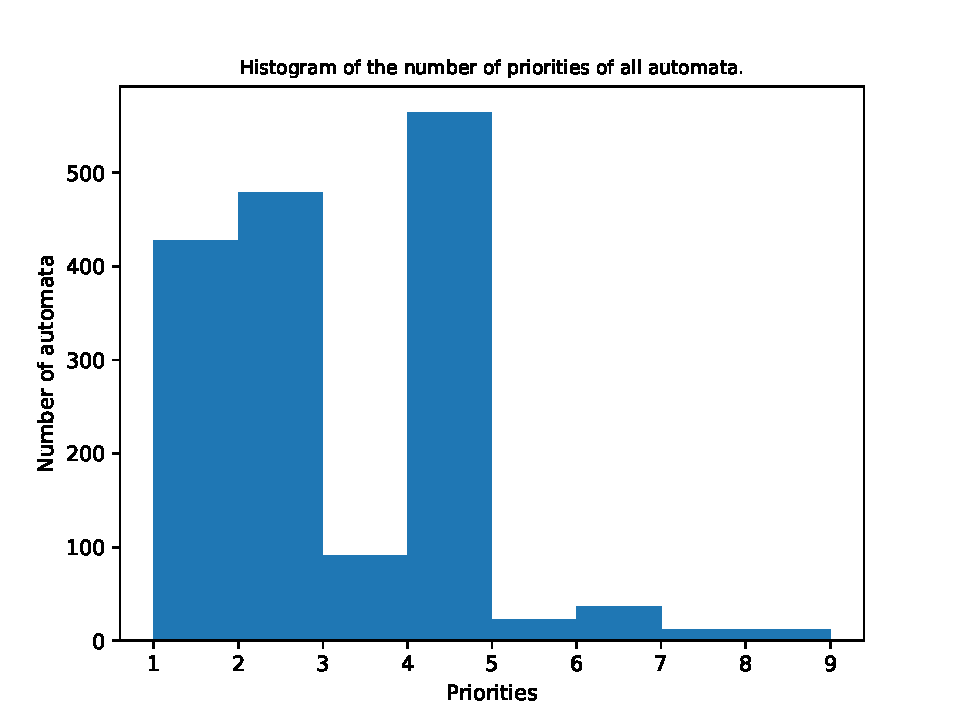
\includepdf{../data/analysis/rawstats.pdf}